\section{Inferentiel databehandling}
\label{sec:inferentiel}
%
Først laves en \textit{Principal Component Analysis} (PCA) analyse på det samlede datasæt, for at se om der er korrelation mellem nogle af de 23 skala spørgsmål. Der laves et screeplot for at se hvor meget af variansen, der forklares af hver \textit{Principal Components} (PC).

\begin{figure}[H]
\centering
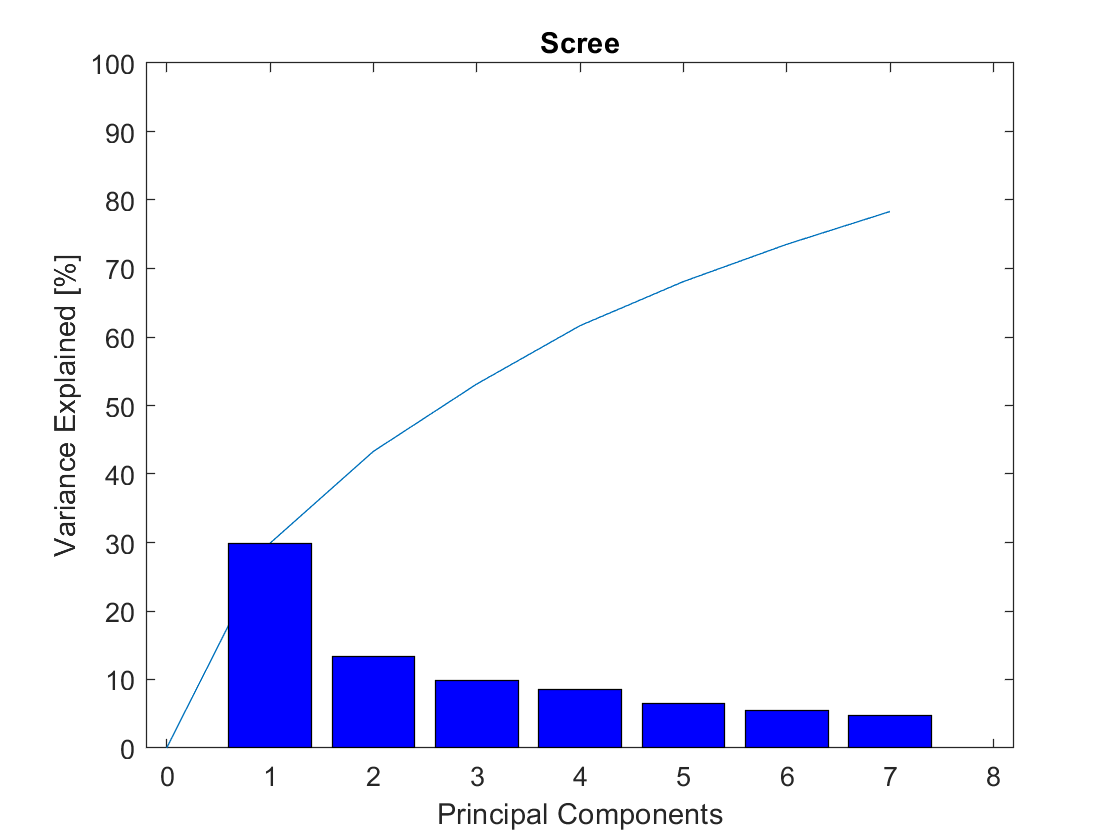
\includegraphics[width=\textwidth]{Figure/DatabehandlingSkalaer/PCAfigures/Scree.png}
\caption{\textit{Scree}-plot, hvorpå sammenhængen mellem antallet af \textit{Principal Components} og \textit{Variance Explained [\%]} fremgår.}
\label{fig:Scree}
\end{figure}
\noindent
%
Ud fra \textit{Scree}-plottet på \autoref{fig:Scree} fremgår det, at der ikke er en tydelig sammenhæng i variansen fra datasættet, da kun 29.9 \% af variansen kan forklares af PC1 og 13.4 \% af PC2. Selv hvis de tre første principal components medregnes, er det kun 53.1 \% af variansen som forklares af modellen. Dette skyldes formentligt, at der ikke er nok data og at for mange variable er blevet varieret på én gang, hvilket har gjort det svært at se hvilke parametre, der har indflydelse på hvilke vurderinger.

Ud fra \textit{Score}-plottet på \autoref{fig:Score} fremgår det også at PC1 kun forklarer en lille del af variansen, da der er meget spredning i datapunkterne og spredningen ikke er systematisk. Hvis PC1 havde forklaret en større del af variansen, ville data være mere centreret omkring den horisontale akse.
%
\begin{figure}[H]
\centering
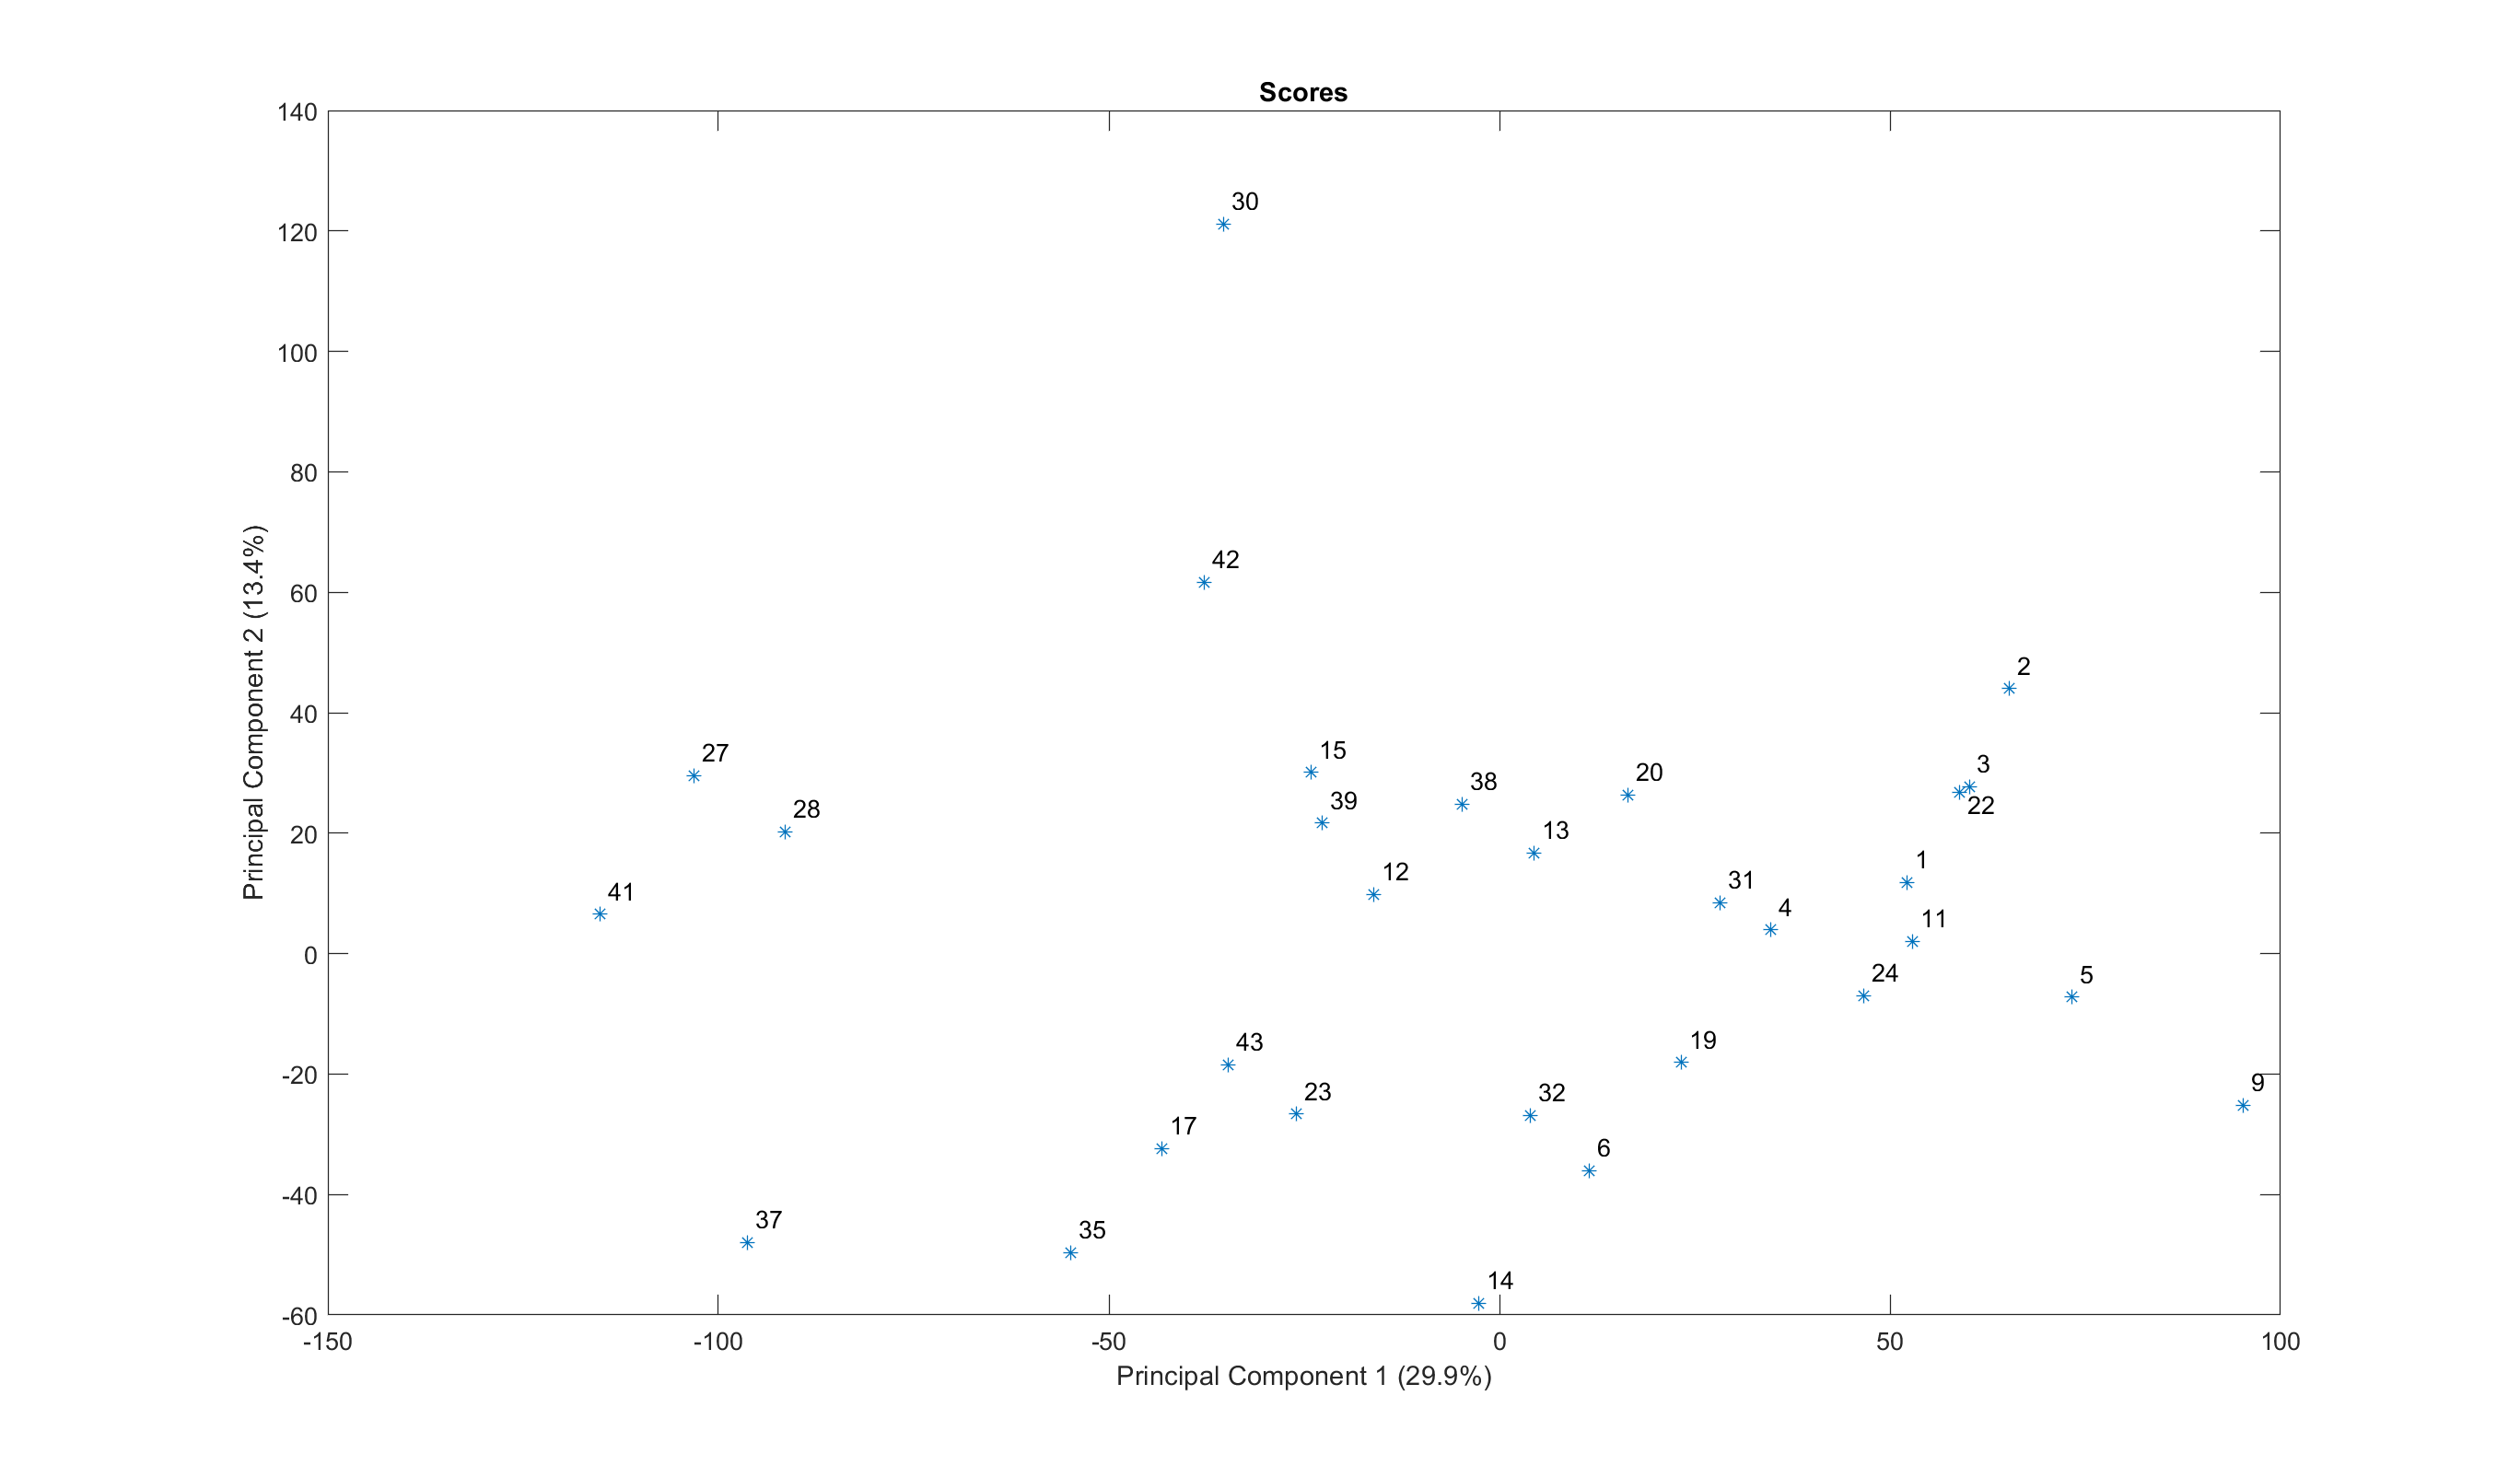
\includegraphics[width=\textwidth]{Figure/DatabehandlingSkalaer/PCAfigures/Scores}
\caption{\textit{Score}-plot for PC1 og PC2.}
\label{fig:Score}
\end{figure}
\noindent
%
For at undersøge hvilke loadings der bidrager til hver principal component, opstilles et biplot, hvori både scores og loadings kan ses. Biplottet på \autoref{fig:Biplot} giver det bedste overblik, da det er nemmest at fortolke i 2D, men 3D plottet er også vedlagt i autoref{ElektroniskBilag3D}, hvor det er muligt at rotere plottet og se det fra forskellige vinkler. Ud fra disse to plots kan det ses at der er korrelation mellem SQ14 og SQ15, SQ17 og SQ22 samt SQ9 og SQ21.
%
\begin{figure}[H]
\centering
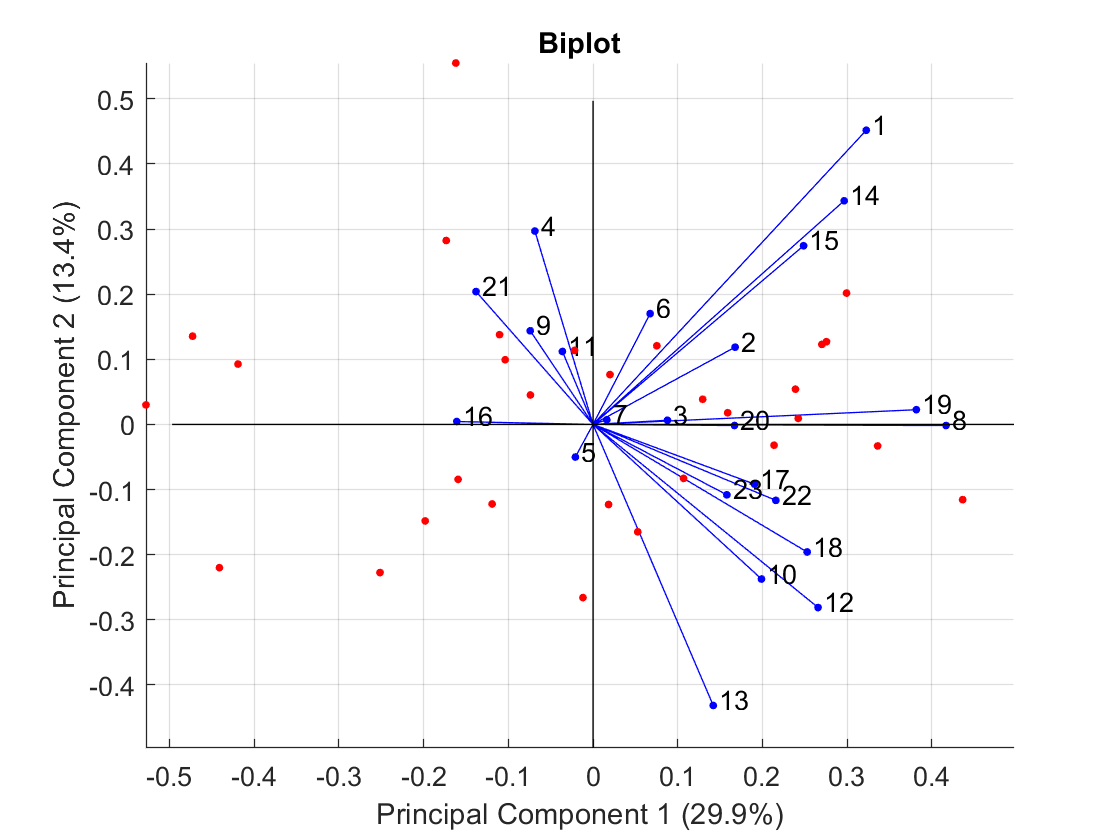
\includegraphics[width=\textwidth]{Figure/DatabehandlingSkalaer/PCAfigures/Biplot}
\caption{\textit{Bi}-plot med både \textit{loadings} (angivet med blå) og \textit{scores} (angivet med rød) fremgår i forhold til robottens højde.}
\label{fig:Biplot}
\end{figure}
\noindent
%
Ud fra 3D plottet kan man se at SQ7 ikke bidrager meget til nogle af de tre PCs. Som nævnt i \fullref{TestAfSkalaVarians} på \autoref{fig:Varians} har SQ7 en meget lille varians, og det er derfor ikke overraskende at den ikke bidrager mere til de tre principal components end den gør resultat er derfor ikke overraskende. Det betyder at spørgsmål 7 har fået nogenlunde samme besvarelser på tværs af grupperne og at den derfor ikke er særlig vigtig for den samlede oplevelse. Det kan dog både være fordi at den ikke er et vigtigt parameter, men det kan også være, at der bare ikke er nogle af testpersonerne, som blev udsat for en oplevelse, der påvirkede dette parameter, men at det måske er vigtigt i andre sammenhænge. 

Resultaterne fra PCA'en fra det samlede datasæt giver ikke nogle håndgribelige konklusioner. For at undersøge om der er nogle tendenser i forhold til de objektive parametre som blev justeret undervejs i testen, højde, retning og afstand, undersøges hvordan hver af disse parametre påvirker en PCA-analyse. Dette gøres ved at kigge på et parameter ad gangen og dele det op i de grupper som allerede findes.